\documentclass{beamer}
\usetheme{Singapore}
\usepackage[round,sort]{natbib}
\usepackage{tikz}
\usetikzlibrary{arrows,decorations.pathmorphing,backgrounds,fit,positioning,shapes.symbols,chains}
\usepackage{adjustbox}
\usepackage{verbatim}
\usepackage{graphicx}
\graphicspath{ {etig-term-paper-presentation-images/} }

\title{The effect of inventor mobility on  invention complexity}
\subtitle{ETIG Course Term Paper}
\author{Ashwin Iyenggar}
\institute[Indian Institute of Management Bangalore] 
{
  Corporate Strategy and Policy\\
  Indian Institute of Management Bangalore
}
\date{10 March, 2017}
\subject{The effect of inventor mobility on  invention complexity\\ETIG Course Term Paper}

% \pgfdeclareimage[height=0.5cm]{university-logo}{university-logo-filename}
% \logo{\pgfuseimage{university-logo}}

\AtBeginSubsection[]
{
  \begin{frame}<beamer>{Outline}
    \tableofcontents[currentsection,currentsubsection]
  \end{frame}
}

\begin{document}

\begin{frame}
  \titlepage
\end{frame}

\begin{frame}{Outline}
  \tableofcontents
  % You might wish to add the option [pausesections]
\end{frame}
\section{Motivation}

\begin{frame}{Mobility Trends}
\begin{figure}[h]
\begin{centering}
  \includegraphics[width=0.7\textwidth]{countrymoves}
  \caption{Country moves by year}
   \label{fig:countrymoves}
\end{centering}
\end{figure}
\end{frame}

\begin{frame}{Mobility Trends}
\begin{figure}[h]
\begin{centering}
  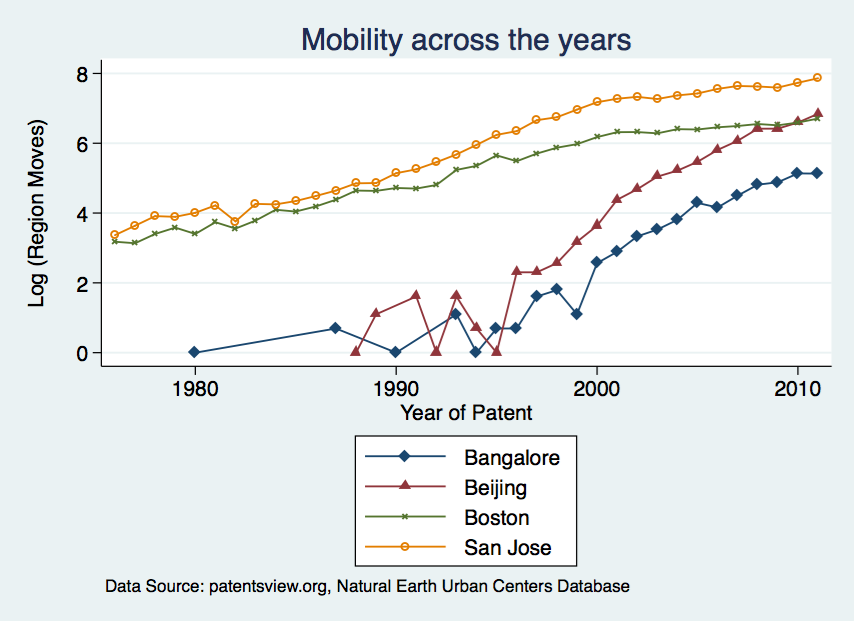
\includegraphics[width=0.7\textwidth]{regionmoves}
  \caption{Region moves by year}
   \label{fig:regionmoves}
\end{centering}
\end{figure}
\end{frame}

\begin{frame}{Mobility Trends}
%------- Begin LaTeX code -------%

\begin{table}[htbp]\centering \caption{Summary statistics \label{sumstat}}
\begin{tabular}{l c c  c}\hline\hline
\multicolumn{1}{c}{\textbf{Variable}} & \textbf{Mean}
 & \textbf{Std. Dev.} & \textbf{N}\\ \hline
moved region & 0.08 & 0.271  & 8537410\\
moved country & 0.029 & 0.166  & 8537410\\
log(complexity) & -1.004 & 2.383  & 7957162\\
inventor pool & 8.542 & 46.674  & 8537410\\
team pool proxy& 27.901 & 112.154  & 6875208\\
\hline
\end{tabular}
\end{table}
%------- End LaTeX code -------%

\end{frame}



\begin{frame}{Research Question}{}
\begin{itemize}
\item{What is the relationship between the movement of some inventors into or out of a region and the average complexity of inventions from those inventors?}
\end{itemize}
\end{frame}

\section{Theory}
\begin{frame}{Hypotheses}{}
\begin{itemize}
\item{H1: An increase in the average mobility of inventors in a region increases the average complexity of  innovation generated}
\item{H2: The effect in H1 is moderated positively by the relative strength of the intellectual property rights regime of the region}
\end{itemize}
\end{frame}



\section{Data and Method}
\begin{frame}{Geographic Mapping}{San Jose}
\begin{figure}[h!]
\begin{centering}
  \includegraphics[width=0.7\textwidth]{SanJose}
  \caption{Geographic Definition of San Jose, CA}
   \label{fig:SanJose}
\end{centering}
\end{figure}
\end{frame}

\begin{frame}{Geographic Mapping}{Bangalore}
\begin{figure}[h!]
\begin{centering}
  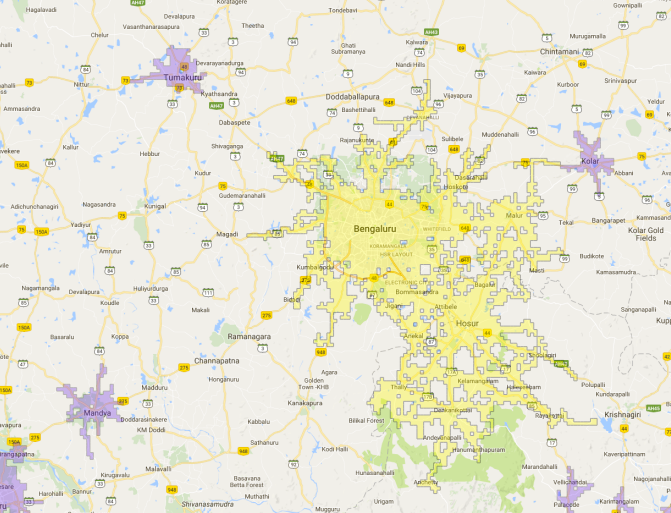
\includegraphics[width=0.7\textwidth]{Bangalore}
  \caption{Geographic Definition of Bangalore}
   \label{fig:Bangalore}
\end{centering}
\end{figure}
\end{frame}

\begin{frame}{Complexity and Technology Classes}
\begin{table}[htbp]\centering \caption{Most complex technology subclasses in 2010 \label{sumstat}}
\begin{tabular}{l c c  c}\hline\hline
\multicolumn{1}{c}{\textbf{id}} & \textbf{Avg Complexity} & \textbf{Technology} \\ \hline
32	&6.691109	&Surgery \& Med Inst.\\
25	&6.583521	&Electronic business methods and software\\
24	&6.361433	&Information Storage\\
22	&5.941292	&Computer Hardware \& Software\\
21	&5.627072	&Communications\\
\hline
\end{tabular}
\end{table}
\end{frame}		

\begin{frame}{Complexity and Technology Classes}		
\begin{table}[htbp]\centering \caption{Least complex technology subclasses in 2010 \label{sumstat}}
\begin{tabular}{l c c  c}\hline\hline
\multicolumn{1}{c}{\textbf{id}} & \textbf{Avg Complexity} & \textbf{Technology} \\ \hline
11	&2.533947	&Agriculture,Food,Textiles\\
33	&3.468262	&Genetics\\
66	&3.488879	&Heating\\
52	&3.518574	&Metal Working\\
63	&3.661588	&Apparel \& Textile\\
53	&3.667615	&Motors \& Engines + Parts\\
55	&3.712974	&Transportation\\
\hline
\end{tabular}
\end{table}
\end{frame}

\begin{frame}{Methodology}{}
\begin{itemize}
\item{Data Source: Patents from USPTO, source: patentsview.org}
\item{Data Source: Regions using Remote Sensing Data, source: naturalearthdata.com}
\item{Unit of Analysis: Inventor-Year}
\item{Dependent Variable: log(Complexity of Invention)}
\item{Primary Explanatory Variable: Mobility of innovators (Between-Region Mobility, Between-Country Mobility)}
\item{Moderating Variable: IPR Strength }
\item{Control Variables: Technology classes, Region-Firm (Assignee) effects, Year effects}
\end{itemize}
\end{frame}

\begin{frame}{Addressing Potential Issues}{}
\begin{itemize}
\item{Direction of Causality}
\item{Alternative measures of complexity }
\item{Cluster Standard Errors at Region - Assignee}
\item{Control for Inventor - Technology Class}
\item{IPR measures - Ginarte Park Index}
\end{itemize}
\end{frame}

\begin{frame}{Results}{}

\end{frame}

\section{Future Work}
\begin{frame}{Limitations and Future Work}{}
\begin{itemize}
\item{Causal forces in determining mobility effects on invention complexity - Learnings from 9/11 shock}
\item{Explore alternate identification measures for causality}
\item{Estimate the extent of under reporting of mobility, consider alternative sources as linkedin}
\item{Industry specific studies with relevant IPR scores}
\item{Alternate measures of complexity}
\end{itemize}
\end{frame}

\bibliography{/Users/aiyenggar/OneDrive/code/bibliography/ae,/Users/aiyenggar/OneDrive/code/bibliography/fj,/Users/aiyenggar/OneDrive/code/bibliography/ko,/Users/aiyenggar/OneDrive/code/bibliography/pt,/Users/aiyenggar/OneDrive/code/bibliography/uz}
\bibliographystyle{apalike}

\end{document}

\begin{comment}
\begin{figure}[h]
\begin{centering}
  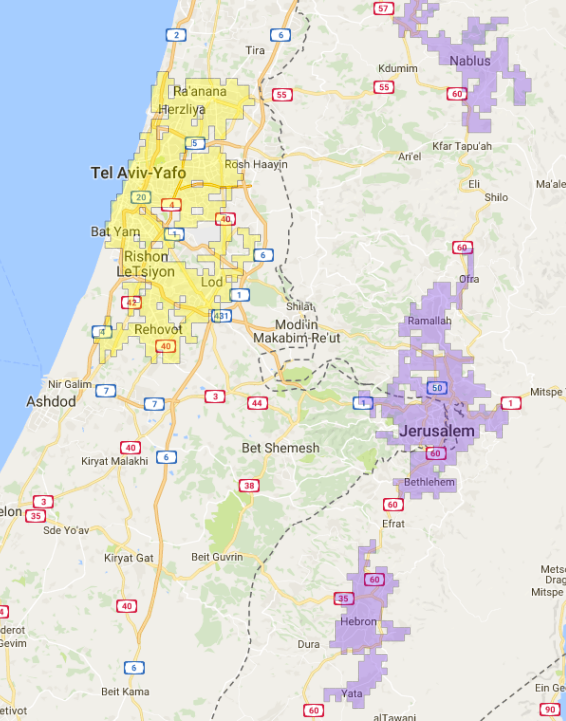
\includegraphics[width=\textwidth]{TelAviv}
  \caption{Geographic Definition of Tel Aviv-Yafo}
   \label{fig:TelAviv}
\end{centering}
\end{figure}
\end{comment}

